\documentclass[UTF8,a4paper,11pt]{ctexart}

\usepackage{amsmath,amssymb,bm,mathtools}
\usepackage{geometry}
\usepackage{booktabs,longtable,tabularx,array,multirow}
\usepackage{enumitem}
\usepackage{xcolor}
\usepackage{hyperref}
\usepackage{cleveref}
\usepackage{tikz}
\usetikzlibrary{arrows.meta,positioning,calc,shapes.geometric,fit}
\usepackage{listings}
\usepackage{caption}
\usepackage{microtype}

\geometry{left=24mm,right=24mm,top=25mm,bottom=25mm}
\setlength{\parindent}{2em}
\setlength{\parskip}{0.25em}
\linespread{1.15}

\definecolor{codegray}{RGB}{248,248,248}
\definecolor{coderule}{RGB}{215,215,215}
\lstset{
  basicstyle=\ttfamily\small,
  backgroundcolor=\color{codegray},
  frame=single,
  rulecolor=\color{coderule},
  breaklines=true,
  columns=fullflexible,
  showstringspaces=false
}

\hypersetup{
  colorlinks=true,
  linkcolor=black,
  citecolor=black,
  urlcolor=blue,
  pdftitle={SI-HHO-Q: QUANTUM Electricity V2 数值方法与实施规范},
  pdfauthor={OpenAI ChatGPT}
}

\newcommand{\R}{\mathbb{R}}
\newcommand{\Pp}{\mathbb{P}}
\newcommand{\dd}{\mathrm{d}}
\newcommand{\jump}[1]{\left[\!\left[#1\right]\!\right]}
\newcommand{\avg}[1]{\left\{\!\left\{#1\right\}\!\right\}}
\newcommand{\eps}{\varepsilon}
\newcommand{\vct}[1]{\bm{#1}}
\newcommand{\T}{\mathsf{T}}
\newcommand{\diag}{\operatorname{diag}}
\newcommand{\Span}{\operatorname{span}}
\newcommand{\argmin}{\operatorname*{arg\,min}}
\newcommand{\norm}[1]{\left\lVert #1\right\rVert}
\newcommand{\ip}[2]{\left(#1,#2\right)}

\title{\bfseries SI-HHO-Q：面向 QUANTUM 电喷雾求解器的\\Sharp-Interface Hybrid High-Order 电学方法\\\large 数值离散、静态消元、守恒通量、BDF2--Schur 电荷耦合与代码映射}
\author{QUANTUM Electricity V2 方法设计稿}
\date{2026年9月}

\begin{document}
\maketitle

\begin{abstract}
本文提出一套用于 QUANTUM 两相电流体（electrohydrodynamics, EHD）求解器的新一代电学离散方法，记为 SI-HHO-Q（Sharp-Interface Hybrid High-Order method with conservative surface charge for QUANTUM）。该方法针对现有 \texttt{sharpHermiteP3} 路径在离散方程级审计中暴露出的结构性问题进行重构：原有方法虽具有严格的有限体积通量守恒、高质量的 Hermite/P3 界面重构以及一致的电流/Maxwell 应力后处理，但非局部 P3 通量修正和 AMR 修正会使全局 Poisson 算子一般失去对称性、正定性、M-matrix 结构和清晰的离散电能解释。新方法保留 Hermite 界面几何、material panel、积分表面电荷和守恒 remap 等已有优势，将背景 quadtree 中被界面切割的单元分解为相子单元，并将 Hermite 界面直接提升为 HHO 骨架上的内部曲面 face。全局电势由对称、强制（coercive）的 HHO 双线性型给出；单元多项式自由度通过静态消元局部去除；自由表面电荷仅作为界面 trace 方程的载荷；两侧法向位移通量由 equilibrated numerical flux 直接恢复；导电电流由同一位移通量乘以 \(\sigma/\eps\) 得到。固定几何下，电势系统对 panel 积分电荷保持严格线性，从而可将 variable-step BDF2 表面电荷更新写成一个真正的 Schur 线性系统，原则上解除现有 \(\Delta t\,\sigma/\eps\) 的显式松弛稳定性限制。本文按 JCP 数值方法论文的组织方式给出连续模型、离散空间、局部重构、稳定化、局部块矩阵、静态消元、全局骨架系统、界面数值通量、表面电荷矩、BDF2--Schur 系统、RZ/AMR/small-cut 处理、Maxwell 应力恢复、QUANTUM 数据结构映射以及验证与验收标准，作为 Electricity V2 的实施规范。
\end{abstract}

\tableofcontents
\newpage

\section{方法定位与设计原则}

QUANTUM 当前 sharp 电学主线可概括为
\[
\text{cell-centered TPFA}
+\text{Hermite/P3 interface flux correction}
+\text{panel-integrated surface charge}.
\]
该结构在局部/全局 Gauss 守恒、界面两侧电场 trace、传导电流和 Maxwell 应力一致性方面具有明显优点，但在修正后的全局矩阵层面，一般不能保证
\[
A=A^{\T},\qquad A\succ0,
\]
也不能保证 M-matrix、离散最大值原理或与 Maxwell 力一致的离散电能结构。其根本原因并非 P3 局部重构本身不准确，而是一个非局部面通量修正以
\[
A_f=\vct{s}_f\vct{d}_f^{\T}
\]
的形式进入两个相邻控制体行，导致高阶界面信息与全局扩散算子的代数结构发生冲突。

因此 SI-HHO-Q 的基本原则是：
\begin{enumerate}[label=\arabic*)]
  \item \textbf{不再使用 P3 修正全局 Poisson 算子。} 高阶信息必须由一个本身稳定的离散框架产生，而不是作为非局部 correction 叠加到 TPFA 上。
  \item \textbf{保留 sharp interface。} 不采用平滑介电常数或 regularized delta function。
  \item \textbf{保留 panel-integrated charge。} 表面自由电荷仍以 \(Q_i=\int_{\Gamma_i}q_s\dd A\) 为守恒未知量。
  \item \textbf{全局算子对称且 coercive。} 目标是得到可由离散能量导出的 SPD 骨架系统，并使用 CG/AMG 类求解器。
  \item \textbf{电势、位移通量、电流和 Maxwell 应力共享同一个离散电场。} 不允许为电流或力单独再差分一套 \(\vct E\)。
  \item \textbf{移除不必要的高阶几何导数。} 电势主求解器不再依赖 \(\kappa_s\)、\(q_s'\)、\(q_s''\)。
  \item \textbf{固定几何下表面电荷--电场耦合按线性问题处理。} 不再使用欠松弛 Picard 迭代。
\end{enumerate}

本文建议生产默认多项式阶次为
\[
\boxed{k=2},
\]
即 cell/face unknown 为二次多项式，局部 potential reconstruction 为三次多项式。

\section{连续电学模型}

\subsection{两相准静电方程}

设液相和气相分别为 \(\Omega^-\) 和 \(\Omega^+\)，界面为
\[
\Gamma=\partial\Omega^-\cap\partial\Omega^+.
\]
单位法向 \(\vct n\) 规定从负相指向正相。准静电场满足
\[
\vct E^\alpha=-\nabla V^\alpha,\qquad
\vct D^\alpha=\eps^\alpha\vct E^\alpha,
\qquad \alpha\in\{-,+\}.
\]
在 bulk 中不求解体自由电荷：
\begin{equation}
-\nabla\cdot\left(\eps^\alpha\nabla V^\alpha\right)=0
\qquad\text{in }\Omega^\alpha.
\label{eq:bulk_poisson}
\end{equation}

界面电势连续：
\begin{equation}
\jump{V}_\Gamma=V^+-V^-=0.
\label{eq:potential_continuity}
\end{equation}
定义
\[
D_n^\alpha=\vct D^\alpha\cdot\vct n,
\]
则自由表面电荷跃迁条件为
\begin{equation}
D_n^+-D_n^-=q_s.
\label{eq:D_jump}
\end{equation}

对于 leaky-dielectric 导电模型，
\begin{equation}
\vct J^\alpha=\sigma^\alpha\vct E^\alpha
=\frac{\sigma^\alpha}{\eps^\alpha}\vct D^\alpha.
\label{eq:ohmic_current}
\end{equation}
本文第一版假定每一相中的 \(\eps^\alpha\) 和 \(\sigma^\alpha\) 在一个时间步内为常数；推广到分片光滑系数只改变局部积分和 current functional 的构造。

\subsection{planar/RZ 统一弱形式}

定义几何权函数
\begin{equation}
m(\vct x)=
\begin{cases}
1, & \text{二维平面问题},\\
2\pi r, & \text{轴对称 }(r,z)\text{ 问题}.
\end{cases}
\label{eq:measure_weight}
\end{equation}
对体和面分别定义
\[
(u,v)_T^m=\int_Tmuv\,\dd A,
\qquad
\langle u,v\rangle_F^m=\int_Fmuv\,\dd s.
\]
在外边界 Dirichlet/Neumann 条件略去记号的情况下，连续弱形式为：求连续跨界面的 \(V\)，使得对所有 admissible test function \(W\)，
\begin{equation}
\boxed{
\sum_{\alpha=\pm}
\int_{\Omega^\alpha}
m\eps^\alpha\nabla V^\alpha\cdot\nabla W^\alpha\,\dd A
=
\int_\Gamma mq_sW\,\dd s
+\ell_{\partial\Omega}(W).
}
\label{eq:weak_form}
\end{equation}
式\eqref{eq:weak_form} 具有两个直接后果：
\begin{itemize}
  \item 表面自由电荷天然是\textbf{界面载荷}，不需要先转换为 cell delta source；
  \item RZ 几何只通过 \(m=2\pi r\) 进入积分，不需要在局部 Taylor 展开中显式出现 \(1/r\) 或 \(1/r^2\)。
\end{itemize}

\section{Hermite 界面诱导的相子单元与骨架网格}

\subsection{从背景 quadtree 到 phase elements}

背景网格仍然采用 QUANTUM 当前 quadtree/Cartesian 叶单元。对于一个背景单元 \(K\)：
\begin{itemize}
  \item 若未被界面切割，则生成一个 HHO element \(T=K\)；
  \item 若被界面切割，则生成
  \[
  T^-=K\cap\Omega^- ,\qquad T^+=K\cap\Omega^+,
  \]
  并将 Hermite panel
  \[
  \Gamma_K=K\cap\Gamma
  \]
  作为 \(T^-\) 和 \(T^+\) 共享的内部 curved skeletal face。
\end{itemize}

\begin{figure}[htbp]
\centering
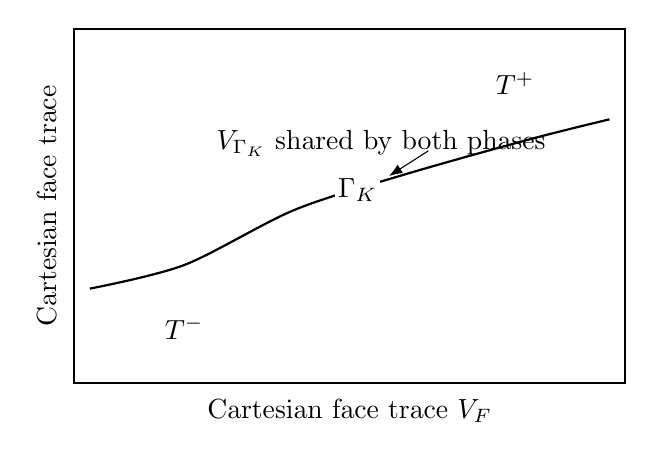
\begin{tikzpicture}[scale=1.0,>=Latex]
  \draw[thick] (0,0) rectangle (7,4.5);
  \draw[thick] plot[smooth] coordinates {(0.2,1.2) (1.4,1.5) (2.8,2.2) (4.2,2.65) (5.8,3.1) (6.8,3.35)};
  \node at (5.6,3.8) {$T^+$};
  \node at (1.4,0.7) {$T^-$};
  \node[fill=white,inner sep=1pt] at (3.6,2.45) {$\Gamma_K$};
  \node at (3.5,-0.35) {Cartesian face trace $V_F$};
  \node[rotate=90] at (-0.35,2.25) {Cartesian face trace};
  \node at (3.9,3.05) {$V_{\Gamma_K}$ shared by both phases};
  \draw[->] (4.5,2.95) -- (4.0,2.63);
\end{tikzpicture}
\caption{SI-HHO-Q 的局部拓扑。Hermite 界面不再作为 P3 correction 的参考几何，而直接成为 HHO skeleton 上的内部曲面 face。}
\label{fig:cut_cell_topology}
\end{figure}

这种处理与标准 unfitted HHO 文献中的 Nitsche/doubled-face 形式并不完全相同。本文方案利用 QUANTUM 已有 Hermite 几何将界面显式提升为骨架 face，因此电势连续条件通过共享 trace 强制满足。标准 unfitted HHO 的稳定性、高反差鲁棒性和 cell agglomeration 结果提供理论参照\cite{BurmanErn2018,BurmanCicuttinDelayErn2021}，但本文 curved shared-trace 变体仍需通过专门的数值验证和后续理论分析确认其最优误差性质。

\subsection{Cartesian face 的 phase splitting}

当一个背景 Cartesian face 被界面切割时，不再将其视为单个电学 face，而按相连通部分生成多个 phase subfaces。例如
\[
F=F^-\cup F^+.
\]
每个最大连通 phase subface 都有独立的骨架 trace，自然避免在同一个 face unknown 中混合两种介质。

\subsection{2:1 AMR coarse--fine 接口}

2:1 quadtree 接口不再使用现有 virtual coarse child + least-squares gradient。若 coarse face 对应两个 fine subfaces，则直接把它们作为两个真实 skeletal faces：
\[
F=F_1\cup F_2.
\]
coarse element 和相邻 fine element 共享对应的 \(F_1,F_2\) face unknown。这样 coarse--fine conservation 由同一全局 face 方程保证，不需要额外的 AMR flux correction。

\section{离散空间与多项式基函数}

本节明确 SI-HHO-Q 的离散未知量、基函数、投影算子及其与局部高阶电势重构之间的关系。需要特别强调：HHO 的局部未知量
\(\underline V_T\) 是一组 \emph{cell/face polynomial data}，并不是一个定义在整个单元上的单一连续函数。真正用于计算梯度、电场和局部能量的是后续重构得到的 \(p_T^{k+1}\underline V_T\)。

\subsection{Phase-element 局部 hybrid unknown}

对任意 phase element \(T\)，记其骨架面集合为 \(\mathcal F_T\)。定义局部 HHO 空间
\begin{equation}
\boxed{
\underline U_T^k
=
\Pp^k(T)\times\prod_{F\in\mathcal F_T}\Pp^k(F),
}
\label{eq:local_hho_space}
\end{equation}
并写局部未知量为
\begin{equation}
\underline V_T
=
\left(V_T,\{V_F\}_{F\in\mathcal F_T}\right),
\label{eq:local_unknown}
\end{equation}
其中
\[
V_T\in\Pp^k(T),\qquad
V_F\in\Pp^k(F).
\]
第一版固定
\[
\boxed{k=2}.
\]
二维中
\[
\dim\Pp^2(T)=6,\qquad
\dim\Pp^2(F)=3.
\]
因此，一个具有 \(N_F\) 条骨架面的 element 具有
\[
6+3N_F
\]
个局部 hybrid DOF。这里 \(V_T\) 主要承载 element 内部多项式信息，\(V_F\) 则承担 element 之间、电极边界以及液气界面上的耦合信息。

\begin{figure}[htbp]
\centering
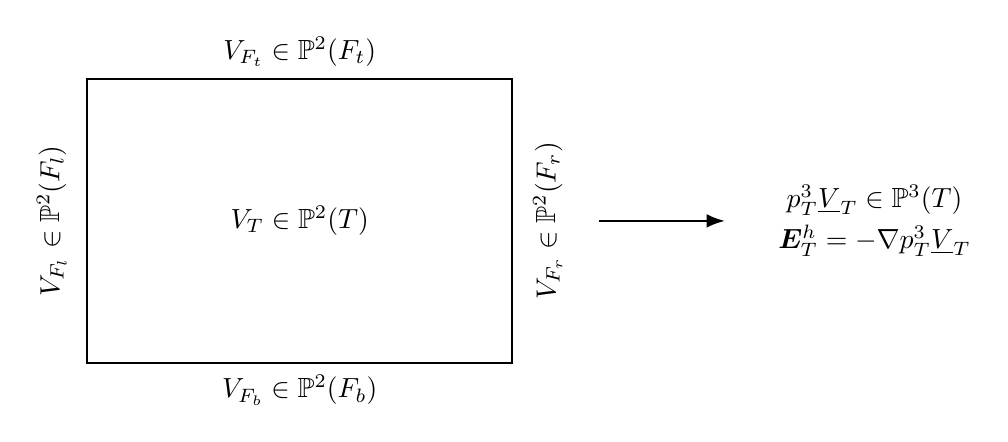
\begin{tikzpicture}[scale=1.0,>=Latex]
  \draw[thick] (0,0) rectangle (5.4,3.6);
  \node at (2.7,1.8) {$V_T\in\Pp^2(T)$};
  \node at (2.7,3.95) {$V_{F_t}\in\Pp^2(F_t)$};
  \node at (2.7,-0.35) {$V_{F_b}\in\Pp^2(F_b)$};
  \node[rotate=90] at (-0.45,1.8) {$V_{F_l}\in\Pp^2(F_l)$};
  \node[rotate=90] at (5.85,1.8) {$V_{F_r}\in\Pp^2(F_r)$};
  \draw[->,thick] (6.5,1.8) -- (8.1,1.8);
  \node[align=center] at (10.0,1.8) {$p_T^3\underline V_T\in\Pp^3(T)$\\[1mm]$\vct E_T^h=-\nabla p_T^3\underline V_T$};
\end{tikzpicture}
\caption{普通四面骨架 element 上的 HHO 局部自由度及其三次电势重构。cell/face unknown 均为二次多项式数据；真正用于局部电场计算的是三次 reconstructed potential。}
\label{fig:hho_local_dofs}
\end{figure}

\subsection{全局 skeleton space 与共享界面 trace}

在全局层面，每一条物理 skeletal face 只有一份 face polynomial unknown。忽略已施加的 Dirichlet face 后，可写
\begin{equation}
\underline U_h^k
=
\left\{
\bigl((V_T)_{T\in\mathcal T_h},(V_F)_{F\in\mathcal F_h}\bigr):
V_T\in\Pp^k(T),\ V_F\in\Pp^k(F)
\right\}.
\label{eq:global_hho_space}
\end{equation}
普通内部 Cartesian subface 由相邻 elements 共享同一个 \(V_F\)。对于 dielectric interface face \(F=\Gamma_i\)，两侧 phase elements 同样共享唯一的
\[
V_{\Gamma_i}\in\Pp^2(\Gamma_i).
\]
因此，离散电势的单值性是在 skeleton unknown 层面强制的：
\[
V_{\Gamma_i}^-\equiv V_{\Gamma_i}^+\equiv V_{\Gamma_i}.
\]
这里需要区分两个概念：共享的是 skeleton trace \(V_{\Gamma_i}\)，而两侧局部 reconstructed potentials 一般并不满足
\[
p_{T^-}^3|_{\Gamma_i}=p_{T^+}^3|_{\Gamma_i}=V_{\Gamma_i}
\]
的逐点恒等式。HHO 是非协调（nonconforming）高阶方法；reconstructed trace 与 skeletal trace 的不一致由第~\ref{sec:stabilization} 节的 stabilization 控制。这个区分对实现非常重要，不能把 \(V_F\) 错误地当作 \(p_T^3\) 的强制 Dirichlet trace。

\subsection{Cell、face 与 reconstruction 基函数}

对 element \(T\)，定义局部长度尺度 \(h_T\) 和几何中心 \((r_T,z_T)\)，使用缩放坐标
\[
\xi=\frac{r-r_T}{h_T},\qquad
\eta=\frac{z-z_T}{h_T}.
\]
第一版可从以下原始 scaled monomial bases 出发：
\begin{align}
\mathcal B_T^2
&=\{1,\xi,\eta,\xi^2,\xi\eta,\eta^2\},\\
\mathcal B_T^3
&=\mathcal B_T^2\cup
\{\xi^3,\xi^2\eta,\xi\eta^2,\eta^3\}.
\end{align}
其中 \(\mathcal B_T^2\) 用于 cell unknown \(V_T\)，\(\mathcal B_T^3\) 用于 reconstructed potential \(p_T^3\)。二者必须作为两套独立 basis 对象保存，不能混用 coefficient vector。

为了降低 cut element、扁长 macro-element 和 near-axis element 上的 conditioning，建议对上述 scaled monomial 做局部 Cholesky/QR 正交化。\textbf{第一版建议 basis conditioning 使用纯几何的、无材料系数的局部 mass matrix}，即不把 \(\eps_T\) 写入 basis normalization；planar/RZ 的物理权重以及 \(\eps_T\) 只进入后续 projector、reconstruction 和 bilinear form。这样 basis identity 不会因介电常数改变而改变，便于 cache、A/B 调试以及高反差材料测试。

对于一维 skeletal face，使用归一化弧长坐标 \(\zeta\in[-1,1]\)。第一版采用 Legendre 型基函数
\begin{equation}
\boxed{
\psi_0=1,\qquad
\psi_1=\zeta,\qquad
\psi_2=\frac12(3\zeta^2-1).
}
\label{eq:face_basis}
\end{equation}
曲线 Hermite interface face 上的 \(\zeta\) 由 panel 局部弧长归一化得到；因此“几何的 Hermite 高阶表示”和“界面电势的 \(\Pp^2\) face basis”是两个不同层次。保持 \(\psi_0\equiv1\) 非常重要，因为后续第 0 个 residual/flux moment 可直接解释为该 face 的积分通量。

\subsection{Reduction/projector：离散数据从何而来}

为说明 polynomial consistency，定义连续函数到 HHO data 的 reduction operator
\begin{equation}
\underline I_T^k v
=
\left(\pi_T^k v,\{\pi_{F,m}^k v\}_{F\in\mathcal F_T}\right).
\label{eq:reduction_operator}
\end{equation}
其中 cell projector 取标准 \(L^2(T)\) projection
\begin{equation}
\int_T\left(\pi_T^k v-v\right)q_k\,\dd A=0
\qquad\forall q_k\in\Pp^k(T),
\label{eq:cell_projection}
\end{equation}
而 face projector 采用与物理面测度一致的加权投影
\begin{equation}
\boxed{
\int_Fm\left(\pi_{F,m}^k v-v\right)q_k\,\dd s=0
\qquad\forall q_k\in\Pp^k(F).
}
\label{eq:weighted_face_projection}
\end{equation}
planar 情形 \(m=1\)，故退化为普通 \(L^2(F)\) projection。RZ 情形使用 \(m=2\pi r\)。在 \(r=0\) 轴面不创建 skeleton DOF，因此无需定义退化的 weighted face projector。

采用“cell 普通投影 + face 加权投影”是有意的。对于常系数 \(\eps_T\)、直 Cartesian element 和 \(w\in\Pp^{k+1}(T)\)，有
\[
\nabla\cdot(m\eps_T\nabla w)\in\Pp^k(T),
\]
而 \(\nabla w\cdot\vct n_{TF}\in\Pp^k(F)\)。因此式\eqref{eq:cell_projection} 与式\eqref{eq:weighted_face_projection} 正好保持后续 weighted Green identity 中的体项和面项。对于 curved Hermite interface，\(\vct n(s)\) 随弧长变化，上述严格 polynomial exactness 不再成立；这属于本方法的 curved-geometry consistency 误差，需要依靠高阶几何 quadrature 和 MMS 收敛测试控制，而不能简单宣称为代数精确。

\subsection{局部维度与实现速查}

对一个普通四面 element、\(k=2\)，主要矩阵维度如表~\ref{tab:hho_local_dimensions}。
\begin{table}[htbp]
\centering
\small
\begin{tabular}{lll}
\toprule
对象 & 含义 & 四面 element 尺寸\\
\midrule
\(V_T\) & cell unknown & 6\\
\(V_F\) & 每条 face trace & 3/face\\
\(\underline V_T\) & local hybrid vector & \(6+4\times3=18\)\\
\(p_T^3\) & reconstructed potential & 10 coefficients\\
\(G_T\) & reconstruction gradient matrix & \(10\times10\)，rank 9\\
增广 reconstruction system & 固定常数模后的局部系统 & \(11\times11\)\\
\(K_{cc}\) & cell--cell block & \(6\times6\)\\
\(K_{cf}\) & cell--face block & \(6\times12\)\\
\(K_{ff}\) & face--face block & \(12\times12\)\\
\(S_T\) & cell-condensed face block & \(12\times12\)\\
\bottomrule
\end{tabular}
\caption{\(k=2\) 普通四面 element 的局部自由度与矩阵尺寸。cut/agglomerated element 只改变 face 数 \(N_F\)，不改变每个 polynomial space 的阶数。}
\label{tab:hho_local_dimensions}
\end{table}

\section{加权局部 HHO potential reconstruction}

\subsection{Weighted Green identity 与重构思想}

HHO 的 potential reconstruction 不是对邻域 cell-center 样本做 least-squares fitting，而是直接由椭圆算子的 Green identity 定义。对任意足够光滑的 \(v,w\)，在一个 phase element \(T\) 上有
\begin{equation}
\boxed{
\int_Tm\eps_T\nabla v\cdot\nabla w\,\dd A
=
-\int_Tv\,\nabla\cdot(m\eps_T\nabla w)\,\dd A
+
\sum_{F\in\mathcal F_T}
\int_Fm\eps_Tv\,\nabla w\cdot\vct n_{TF}\,\dd s .
}
\label{eq:weighted_green_identity}
\end{equation}
HHO 用 cell polynomial \(V_T\) 替代体积分中的 \(v\)，用 face polynomial \(V_F\) 替代边界项中的 trace \(v|_F\)，并寻找一个更高一阶的 polynomial，使其 weighted weak gradient 与这些离散数据一致。因此该 reconstruction 是一个 \emph{variational/PDE-consistent local reconstruction}，而不是旧 Hermite/P3 路径中的 sampling/regression reconstruction。

RZ 情形的关键在于权重必须完整保留在散度内部：
\[
\nabla\cdot(m\eps\nabla w),\qquad m=2\pi r.
\]
对常系数 \(\eps\) 展开可得
\[
\nabla\cdot(2\pi r\eps\nabla w)
=2\pi r\eps\left(w_{rr}+\frac1r w_r+w_{zz}\right),
\]
因此轴对称强形式中的 \((1/r)w_r\) 已经由 weighted weak form 自动包含，不需要另行构造 \(1/r\) 或 \(1/r^2\) 的 Taylor 修正。

\subsection{重构定义与唯一性}

对每个 phase element \(T\)，定义
\[
p_T^{k+1}\underline V_T\in\Pp^{k+1}(T)
\]
使得对所有 \(w\in\Pp^{k+1}(T)\)（模去常数）
\begin{equation}
\boxed{
\begin{aligned}
\int_Tm\eps_T\nabla p_T^{k+1}\underline V_T\cdot\nabla w\,\dd A
=&-
\int_TV_T\nabla\cdot\left(m\eps_T\nabla w\right)\,\dd A\\
&+\sum_{F\in\mathcal F_T}
\int_Fm\eps_TV_F\nabla w\cdot\vct n_{TF}\,\dd s .
\end{aligned}
}
\label{eq:local_reconstruction}
\end{equation}
由于式\eqref{eq:local_reconstruction} 只确定梯度，还需要一个平均值条件固定常数模：
\begin{equation}
\boxed{
\int_Tm\,p_T^{k+1}\underline V_T\,\dd A
=
\int_Tm\,V_T\,\dd A.
}
\label{eq:mean_constraint}
\end{equation}
对第一版 \(k=2\)，重构结果为
\[
\boxed{p_T^3\underline V_T\in\Pp^3(T)},
\]
因此局部 reconstructed electric field
\[
\vct E_T^h=-\nabla p_T^3\underline V_T
\]
是二次 polynomial vector field。

\subsection{显式增广矩阵系统}

设 \(\{\chi_a\}_{a=1}^{10}\) 为 \(\Pp^3(T)\) basis，\(\{\phi_i\}_{i=1}^{6}\) 为 \(\Pp^2(T)\) cell basis。写
\[
p_T^3\underline V_T=\sum_{a=1}^{10}p_a\chi_a.
\]
定义 gradient Gram matrix
\begin{equation}
(G_T)_{ab}
=
\int_Tm\eps_T\nabla\chi_a\cdot\nabla\chi_b\,\dd A,
\label{eq:G_matrix}
\end{equation}
cell coupling
\begin{equation}
(B_T^c)_{ai}
=-\int_T\phi_i\nabla\cdot(m\eps_T\nabla\chi_a)\,\dd A,
\label{eq:Bc_matrix}
\end{equation}
以及每个 face 的 coupling
\begin{equation}
(B_T^F)_{aj}
=
\int_Fm\eps_T\psi_j^F\nabla\chi_a\cdot\vct n_{TF}\,\dd s.
\label{eq:Bf_matrix}
\end{equation}
将所有 cell/face coupling 横向拼接为 \(B_T\)。再定义 weighted mean vectors
\begin{equation}
(\vct\mu_T)_a=\int_Tm\chi_a\,\dd A,
\qquad
(\vct c_T)_i=\int_Tm\phi_i\,\dd A.
\label{eq:mean_vectors}
\end{equation}
则 reconstruction 不应直接对奇异的 \(G_T\) 做 Cholesky。由于常数 polynomial 属于其 kernel，\(k=2\) 时
\[
\operatorname{rank}(G_T)=9.
\]
实际应解以下 \(11\times11\) 增广系统：
\begin{equation}
\boxed{
\begin{bmatrix}
G_T & \vct\mu_T\\
\vct\mu_T^{\T} & 0
\end{bmatrix}
\begin{bmatrix}
\vct p_T\\ \lambda_T
\end{bmatrix}
=
\begin{bmatrix}
B_T\underline{\vct V}_T\\
\vct c_T^{\T}\vct V_T
\end{bmatrix}.
}
\label{eq:augmented_reconstruction}
\end{equation}
建议对该对称不定小矩阵使用 dense pivoted LDL\(^{\T}\) 或 QR，而不是对 \(G_T\) 本身使用 LLT。固定 geometry/material/basis 后，式\eqref{eq:augmented_reconstruction} 可预计算为线性映射
\begin{equation}
\boxed{
\vct p_T=R_T\underline{\vct V}_T.
}
\label{eq:R_matrix}
\end{equation}
因此运行时 reconstruction 只是一个小型 dense matrix--vector product，而不是重新搜索 stencil 或做邻域拟合。

\subsection{Polynomial consistency 与高一阶重构}

定义式\eqref{eq:reduction_operator} 的 reduction data。对于 planar 或 RZ 的\textbf{直 Cartesian element}、相内常数 \(\eps_T\)、充分精确的积分，以及 \(v\in\Pp^{k+1}(T)\)，weighted Green identity 与 projector 定义给出
\begin{equation}
\boxed{
p_T^{k+1}\underline I_T^k v=v.}
\label{eq:polynomial_reproduction}
\end{equation}
更一般地，\(p_T^{k+1}\underline I_T^k v\) 可解释为相应 weighted elliptic projector。对本文 \(k=2\) 而言，式\eqref{eq:polynomial_reproduction} 表明：\(P^2\) cell/face data 并不是“凭空升阶”，而是利用 cell data 与所有 face data 所携带的总信息，通过局部 Green identity 精确恢复目标空间中的三次 polynomial。

该性质应成为 P0 阶段的硬 patch test：随机生成 \(v\in\Pp^3(T)\)，构造 \(\underline I_T^2v\)，要求 reconstructed coefficients、gradient 和 face energy residual 在直单元上达到舍入误差量级。对于 curved Hermite interface element，由于曲线法向和几何映射使 boundary functional 不再严格属于有限阶 polynomial test space，式\eqref{eq:polynomial_reproduction} 不应未经证明直接宣称；其实际设计阶必须由 curved-interface MMS 验证。

\subsection{RZ 近轴性质}

RZ reconstruction 的能量半范数为
\[
\norm{\nabla v}_{m,\eps,T}^2
=
\int_T2\pi r\,\eps_T|\nabla v|^2\,\dd r\dd z.
\]
在 \(r=0\) 上权重自然退化为零，因此弱形式本身没有强形式 \(1/r\) 项的数值奇点。轴面不创建 face DOF；near-axis element 仍通过 phase-volume quadrature 对 \(2\pi r\) 权重直接积分。需要注意，权重退化会改变局部矩阵尺度，因此 basis normalization、quadrature 误差和 \(K_{cc}\) conditioning 必须在 V9 RZ verification 中单独监控。

\section{稳定化与局部双线性型}
\label{sec:stabilization}

\subsection{为什么需要 stabilization}

局部 reconstructed potential \(p_T^{k+1}\underline V_T\) 与独立 skeletal unknown \(V_F\) 是两个不同对象，一般并不满足逐点
\[
p_T^{k+1}\underline V_T|_F=V_F.
\]
如果只保留 gradient reconstruction energy，某些 cell/face 相对模式可能不被充分控制。HHO stabilization 的作用就是控制这种“skeletal trace 与 reconstructed cell trace 的不一致部分”。它不是为 Poisson 方程人为添加数值黏性，而是补足 hybrid 离散空间中 reconstruction 半范数没有控制到的自由度，同时保持 polynomial consistency、对称性和非负性。

\subsection{Cell/face residual operators}

定义
\begin{align}
\delta_T^k\underline V_T
&=\pi_T^k\left(p_T^{k+1}\underline V_T-V_T\right),\\
\delta_{TF}^k\underline V_T
&=\pi_{F,m}^k\left(p_T^{k+1}\underline V_T-V_F\right).
\end{align}
将 cell correction trace 到 face 后，定义
\begin{equation}
\boxed{
\Delta_{TF}^k\underline V_T
=
\delta_{TF}^k\underline V_T
-
\left(\delta_T^k\underline V_T\right)|_F.
}
\label{eq:stabilization_residual}
\end{equation}
对于一个来自目标 polynomial space 的精确 reduction，理想 straight-element 情形下该 residual 为零，因此 stabilization 不破坏式\eqref{eq:polynomial_reproduction} 的 polynomial consistency。

\subsection{Stabilization 双线性型}

第一版采用
\begin{equation}
\boxed{
 s_T(\underline U_T,\underline V_T)
 =\sum_{F\in\mathcal F_T}
 \eta_T\frac{\eps_T}{h_F}
 \int_Fm\,
 \Delta_{TF}^k\underline U_T
 \Delta_{TF}^k\underline V_T\,\dd s,
}
\label{eq:stabilization}
\end{equation}
默认 \(\eta_T=1\)。尺度 \(\eps_T/h_F\) 与 diffusion energy 的量纲一致。参数 \(\eta_T\in[0.5,4]\) 应在验证阶段做灵敏度测试；若需要通过过大的 \(\eta_T\) 才能维持稳定，优先怀疑 small-cut conditioning、quadrature 或 basis scaling，而不是简单继续增大 penalty。

式\eqref{eq:stabilization} 满足
\[
s_T(\underline U_T,\underline V_T)
=s_T(\underline V_T,\underline U_T),
\qquad
s_T(\underline V_T,\underline V_T)\ge0.
\]
当所有 cell/face DOF 对应同一个常数 \(C\) 时，重构为 \(p_T=C\)，所有 \(\Delta_{TF}^k=0\)。因此 stabilization 精确保留常势零场模式。

\subsection{局部 electrostatic energy 与矩阵}

定义
\begin{equation}
\boxed{
 a_T(\underline U_T,\underline V_T)
 =
 \int_Tm\eps_T
 \nabla p_T^{k+1}\underline U_T\cdot
 \nabla p_T^{k+1}\underline V_T\,\dd A
 +s_T(\underline U_T,\underline V_T).
}
\label{eq:local_bilinear}
\end{equation}
若 \(R_T\) 是式\eqref{eq:R_matrix} 的 reconstruction matrix，\(S_T^{\rm stab}\) 表示 stabilization matrix，则局部矩阵为
\begin{equation}
\boxed{
K_T=R_T^{\T}G_TR_T+S_T^{\rm stab}.
}
\label{eq:local_matrix}
\end{equation}
为避免与后续 static-condensed Schur block \(S_T\) 混淆，本文以下把 stabilization matrix 明确记为 \(S_T^{\rm stab}\)。在 exact arithmetic 下
\[
K_T=K_T^{\T},\qquad
\underline{\vct v}_T^{\T}K_T\underline{\vct v}_T\ge0.
\]
常势模式是局部核；存在全局 Dirichlet anchor 后，该核在全局系统中被去除。这个“gradient reconstruction energy + symmetric positive stabilization”的构造，是 SI-HHO-Q 相比现有 nonlocal P3 flux correction 能恢复对称能量结构的根本原因。

\section{局部块矩阵与静态消元}

\subsection{块结构}

将局部 unknown 分为 cell modes 和 face modes：
\[
\underline{\vct V}_T=
\begin{bmatrix}
\vct V_c\\ \vct V_f
\end{bmatrix}.
\]
对应
\begin{equation}
K_T=
\begin{bmatrix}
K_{cc}&K_{cf}\\
K_{fc}&K_{ff}
\end{bmatrix},
\qquad K_{fc}=K_{cf}^{\T}.
\label{eq:block_matrix}
\end{equation}
对 \(k=2\)，二维单元块
\[
K_{cc}\in\R^{6\times6}.
\]
当前 bulk 无体自由电荷，因此通常 cell RHS \(\vct f_c=0\)。

\subsection{只消元 cell DOF}

Electricity V2 第一版明确规定：\textbf{只静态消元 cell polynomial，自由保留 Cartesian face trace 和 interface trace。} 由
\[
K_{cc}\vct V_c+K_{cf}\vct V_f=\vct f_c
\]
得到
\begin{equation}
\boxed{
\vct V_c=K_{cc}^{-1}\left(\vct f_c-K_{cf}\vct V_f\right).
}
\label{eq:cell_recovery}
\end{equation}
代入 face rows 得
\begin{equation}
\boxed{
S_T\vct V_f=\vct g_T,
}
\label{eq:local_schur}
\end{equation}
其中
\begin{align}
\boxed{S_T}&=K_{ff}-K_{fc}K_{cc}^{-1}K_{cf},\label{eq:local_condensed_matrix}\\
\boxed{\vct g_T}&=\vct f_f-K_{fc}K_{cc}^{-1}\vct f_c.\label{eq:local_condensed_rhs}
\end{align}
不显式形成 \(K_{cc}^{-1}\)。每个 element 保存 dense Cholesky
\[
K_{cc}=L_TL_T^{\T},
\]
通过 triangular solves 构造 \(K_{cc}^{-1}K_{cf}\) 和 cell recovery operator。

因为 Schur complement 保持对称正性，\(S_T\) 仍为对称半正定矩阵。

\section{全局骨架系统与边界条件}

\subsection{全局未知量}

静态消元后，global unknown 仅包含
\[
\boxed{
\text{Cartesian phase-subface traces}
+\text{Hermite interface traces}.
}
\]
记 free skeleton vector 为 \(\vct u\)。全局装配得到
\begin{equation}
\boxed{
S\vct u=\vct d+B_\Gamma\vct\eta,
}
\label{eq:global_skeleton}
\end{equation}
其中 \(\vct d\) 收集 prescribed electrode/boundary contribution，\(\vct\eta\) 是所有 interface charge moments。只要每个局部块 coercive、small cut 已被稳定处理且存在 Dirichlet anchor，则应有
\begin{equation}
\boxed{S=S^{\T}\succ0.}
\label{eq:SPD}
\end{equation}
这使 sharp 电势主系统可使用 PCG/AMG，而不再需要 nonsymmetric SuperLU。

\subsection{Dirichlet 电极}

对 \(V=V_D\) 的 face，直接将 face polynomial 设置为 \(V_D\) 的 \(P^2\) 投影。若 \(V_D\) 为常数，则只有 \(\psi_0\) 模式非零。矩阵按 free/prescribed partition 消元：
\[
S_{ff}\vct u_f
=\vct b_f-S_{fD}\vct u_D.
\]

\subsection{Neumann 与轴面}

homogeneous Neumann face 保留为自由 skeletal unknown，其 global face equation 自然给出零 numerical flux。

在 RZ 对称轴 \(r=0\) 上，物理 measure \(m=2\pi r\) 为零。为避免产生零质量、零能量的孤立 DOF，规定：
\begin{equation}
\boxed{r=0\text{ 轴面不创建 skeleton DOF，直接作为 natural symmetry boundary。}}
\label{eq:axis_rule}
\end{equation}

\section{表面电荷的守恒矩表示}

\subsection{继续保留 panel-integrated charge}

对 Hermite material panel \(\Gamma_i\)，保留
\begin{equation}
\boxed{
Q_i=\int_{\Gamma_i}q_s\,\dd A
=\int_{\Gamma_i}m q_s\,\dd s.
}
\label{eq:panel_charge}
\end{equation}
这仍然是唯一的时间推进守恒未知量。界面拉伸通过 panel physical measure 的改变自然反映到密度 \(q_s=Q_i/A_i\)，不额外重复加入 stretching source。

\subsection{界面载荷矩}

对 interface basis \(\{\psi_a\}_{a=0}^2\)，定义
\begin{equation}
\eta_{i,a}
=\int_{\Gamma_i}m q_h\psi_a\,\dd s.
\label{eq:charge_moments}
\end{equation}
第 0 模式必须严格满足
\begin{equation}
\boxed{\eta_{i,0}=Q_i.}
\label{eq:charge_constant_moment}
\end{equation}
高阶 moments 可继续利用现有 \texttt{SurfaceChargeField} 的局部 quadratic density reconstruction 计算，但不再需要显式输出 \(q_s'\) 和 \(q_s''\)。

由于 reconstruction 对 \(\vct Q\) 为线性映射，可预装配为
\begin{equation}
\boxed{\vct\eta=P_Q\vct Q.}
\label{eq:PQ}
\end{equation}
普通 panel 的高阶 moment 仅依赖相邻少量 panel，因此 \(P_Q\) 是稀疏带状算子；常数模式所在行应直接写成 identity，以避免积分舍入破坏总电荷。

\section{equilibrated numerical flux 与 Gauss 守恒}

\subsection{局部 face residual}

恢复 cell unknown 后，完整局部 face residual 可写为
\begin{equation}
\vct r_{T,f}
=K_{fc}\vct V_c+K_{ff}\vct V_f-\vct f_f.
\label{eq:face_residual_full}
\end{equation}
若 cell 已静态消元，则等价地
\begin{equation}
\vct r_{T,f}=S_T\vct V_f-\vct g_T.
\label{eq:face_residual_condensed}
\end{equation}
定义 face mass matrix
\begin{equation}
(M_F^m)_{ab}=\int_Fm\psi_a\psi_b\,\dd s.
\label{eq:face_mass}
\end{equation}
并定义 numerical primal flux polynomial \(\widehat g_{T,F}\in\Pp^2(F)\) 为
\begin{equation}
\boxed{
M_F^m\widehat{\vct g}_{T,F}=\vct r_{T,F}.
}
\label{eq:primal_flux}
\end{equation}
其物理意义为
\[
\widehat g_{T,F}\approx \eps_T\nabla V\cdot\vct n_{TF}.
\]
对应外法向位移通量为
\[
\widehat D_{T,F}^{\mathrm{out}}=-\widehat g_{T,F}.
\]

\subsection{普通内部 face}

若 \(F\) 被 \(T_1,T_2\) 共享，则同一个 global trace row 给出
\begin{equation}
\boxed{
\vct r_{T_1,F}+\vct r_{T_2,F}=\vct0,
}
\label{eq:internal_flux_balance}
\end{equation}
因此三个 \(P^2\) flux moments 均严格平衡，而不只是积分通量平衡。

\subsection{界面 face 与位移跳跃}

在界面 \(\Gamma_i\) 上，negative phase outward normal 为 \(+\vct n\)，positive phase outward normal 为 \(-\vct n\)。global interface row 为
\begin{equation}
\boxed{
\vct r^-_{\Gamma_i}+\vct r^+_{\Gamma_i}=\vct\eta_i.
}
\label{eq:interface_row}
\end{equation}
又有
\[
r^-\approx\eps^-\nabla V^-\cdot\vct n=-D_n^-,
\]
\[
r^+\approx\eps^+\nabla V^+\cdot(-\vct n)=D_n^+,
\]
所以
\begin{equation}
\boxed{D_n^+-D_n^-=q_h}
\label{eq:discrete_D_jump}
\end{equation}
在整个 \(P^2(\Gamma_i)\) moment space 中成立。

因此建议定义
\begin{equation}
\boxed{
\widehat D_n^-=-\widehat g^-_{\Gamma_i},
\qquad
\widehat D_n^+=+\widehat g^+_{\Gamma_i}.
}
\label{eq:D_traces}
\end{equation}
不再通过后处理令 \(D_n^+=D_n^-+q_s\)。

\subsection{局部与全局 Gauss law}

每个 phase element 在 bulk 中应满足
\begin{equation}
\boxed{
\sum_{F\in\partial T}
\int_F\widehat{\vct D}\cdot\vct n_{TF}\,\dd A=0.
}
\label{eq:local_gauss}
\end{equation}
在 basis \(\psi_0=1\) 下，这等价于所有 face 第 0 residual moment 的代数和为零。

所有内部 Cartesian faces 互相抵消，所有 interface faces 贡献 \(Q_i\)，从而得到全局离散 Gauss closure：
\begin{equation}
\boxed{
\sum_{F\subset\partial\Omega}
\int_F\vct D\cdot\vct n\,\dd A
-
\sum_iQ_i=0.
}
\label{eq:global_gauss}
\end{equation}
该式应作为 runtime hard diagnostic，而不是仅依赖 linear-system residual。

\section{导电电流算子}

由\eqref{eq:ohmic_current}，定义
\[
\rho^\alpha=\frac{\sigma^\alpha}{\eps^\alpha}.
\]
则界面两侧
\[
J_n^-=\rho^-D_n^-,\qquad
J_n^+=\rho^+D_n^+.
\]
沿用现有 QUANTUM 表面电荷符号约定，进入 material panel 的积分法向电流为
\begin{equation}
I_i=\int_{\Gamma_i}(J_n^--J_n^+)\,\dd A.
\label{eq:panel_current_def}
\end{equation}
利用 \(\psi_0=1\) 和式\eqref{eq:D_traces}，直接得到
\begin{equation}
\boxed{
I_i
=-\rho^-r^-_{i,0}
-\rho^+r^+_{i,0}.
}
\label{eq:panel_current_residual}
\end{equation}
因此新方法不再需要：
\begin{itemize}
  \item P3 phase electric-flux split；
  \item displacement split remainder correction；
  \item cell-integrated current；
  \item \texttt{SurfaceChargeField::mapNormalCurrent()} 的按面积 panel 分配。
\end{itemize}
每个 Hermite panel 的电流直接由其两侧 HHO interface residual 得到。

固定 geometry 后，panel current 对 skeleton potential 是 affine map：
\begin{equation}
\boxed{
\vct I=C\vct u+\vct c_D.
}
\label{eq:current_operator}
\end{equation}
其中 \(C\) 可在 prepared operator 阶段由 local condensed blocks 直接组装。

\section{固定几何下的线性电荷--电势结构}

由全局电势方程\eqref{eq:global_skeleton} 与 \(\vct\eta=P_Q\vct Q\)，
\begin{equation}
\boxed{
S\vct u=\vct d+B_\Gamma P_Q\vct Q.
}
\label{eq:potential_charge_system}
\end{equation}
于是
\begin{equation}
\vct u(\vct Q)=S^{-1}\left(\vct d+B_\Gamma P_Q\vct Q\right).
\label{eq:u_of_Q}
\end{equation}
代入式\eqref{eq:current_operator}：
\begin{equation}
\boxed{
\vct I(\vct Q)=\vct I_0+M\vct Q,
}
\label{eq:I_affine_Q}
\end{equation}
其中
\begin{align}
\vct I_0&=\vct c_D+CS^{-1}\vct d,\label{eq:I0}\\
M&=CS^{-1}B_\Gamma P_Q.\label{eq:M_operator}
\end{align}
这是 SI-HHO-Q 时间离散的核心：\textbf{固定 geometry/material 时，所谓 ``charge--electric nonlinear iteration'' 实际上是严格的线性 affine map。}

\section{Variable-step BDF2--Schur 表面电荷系统}

\subsection{时间离散}

经过 fluid/material interface motion 后，首先将历史 charge 保守 remap 到新 geometry，记仍为 \(Q^n,Q^{n-1}\)。设
\[
r_n=\frac{\Delta t_n}{\Delta t_{n-1}}.
\]
variable-step BDF2 系数为
\begin{align}
a_0&=\frac{1+2r_n}{1+r_n},\\
a_1&=-(1+r_n),\\
a_2&=\frac{r_n^2}{1+r_n}.
\end{align}
在不重复计入 material stretching 和 tangential transport 的情况下，电荷松弛方程写为
\begin{equation}
\boxed{
\frac{a_0\vct Q^{n+1}+a_1\vct Q^n+a_2\vct Q^{n-1}}{\Delta t_n}
=\vct I(\vct Q^{n+1}).
}
\label{eq:bdf2_charge}
\end{equation}
当 \(r_n=1\) 时即标准 BDF2。

\subsection{Schur 线性系统}

代入式\eqref{eq:I_affine_Q} 得
\begin{equation}
\boxed{
\left(a_0I-\Delta t_nM\right)\vct Q^{n+1}
=-a_1\vct Q^n-a_2\vct Q^{n-1}
+\Delta t_n\vct I_0.
}
\label{eq:charge_schur}
\end{equation}
第一时间步采用 backward Euler：
\begin{equation}
\boxed{
\left(I-\Delta tM\right)\vct Q^{n+1}
=\vct Q^n+\Delta t\vct I_0.
}
\label{eq:BE_charge}
\end{equation}
因此新路径中删除现有欠松弛 Picard
\[
Q^{m+1}=Q^m-\omega R/\alpha,
\]
并原则上移除
\[
\Delta t\max(\sigma/\eps)\le0.25
\]
作为\textbf{稳定性硬限制}。大时间步仍可能降低时间精度或放大 EHD 强耦合误差，但不应再由显式 dielectric-relaxation stability 约束决定。

\subsection{Matrix-free Schur action}

不显式形成 dense/nonlocal \(M\)。对 trial vector \(\vct x\)，执行
\begin{equation}
\vct x
\xrightarrow{P_Q}
P_Q\vct x
\xrightarrow{B_\Gamma}
\vct b
\xrightarrow{S^{-1}}
\vct y
\xrightarrow{C}
M\vct x.
\label{eq:matrix_free_action}
\end{equation}
因此外层 Schur 系统可用 GMRES；每次 matvec 内部只需要一次 SPD electric solve。二维 verification 阶段可使用 sparse Cholesky/LDLT，production 阶段使用 PCG + IC/AMG，并复用整个时间步中的 preconditioner/hierarchy。

\section{Maxwell 应力恢复}

\subsection{法向场}

法向位移直接采用 equilibrated interface flux：
\[
D_n^-=-\widehat g^-_\Gamma,
\qquad
D_n^+=+\widehat g^+_\Gamma.
\]
因此 \(D_n^+-D_n^-=q_h\) 与 Poisson solve 同源，不再需要 P3 后处理。

\subsection{共同切向场}

对 \(k=2\)，两侧均有 cubic local potential reconstruction
\[
p_{T^-}^3,
\qquad
p_{T^+}^3.
\]
interface skeleton 已有共同二次 trace \(V_\Gamma^2\)。为得到唯一的高质量 tangential field，建议构造共同 cubic interface potential
\[
\widetilde V_\Gamma^3\in\Pp^3(\Gamma)
\]
满足
\begin{equation}
\boxed{
\pi_\Gamma^2\widetilde V_\Gamma^3=V_\Gamma^2.
}
\label{eq:cubic_trace_constraint}
\end{equation}
剩余一个 cubic mode 通过
\begin{equation}
\widetilde V_\Gamma^3
=\argmin_{w\in\Pp^3,\ \pi_\Gamma^2w=V_\Gamma^2}
\left(
\omega^-\norm{w-p_-^3}_{\Gamma,m}^2
+\omega^+\norm{w-p_+^3}_{\Gamma,m}^2
\right)
\label{eq:common_cubic_trace}
\end{equation}
确定。数值上只需一个 \(1\times1\) solve。随后
\begin{equation}
\boxed{E_t^h=-\partial_s\widetilde V_\Gamma^3.}
\label{eq:tangential_field}
\end{equation}
这使旧 P3 中的 \(V_\Gamma,E_t,D_n,E_{t,s},D_{n,s},\ldots\) 一体化拟合被拆解为三个更清晰的来源：
\[
V_\Gamma\leftarrow\text{global shared trace},
\]
\[
D_n^\pm\leftarrow\text{equilibrated HHO flux},
\]
\[
E_t\leftarrow\text{common cubic trace derivative}.
\]
不再需要 \(\kappa_s,q_s',q_s''\)。

\subsection{Maxwell traction}

沿用连续物理公式：
\begin{equation}
\boxed{
\tau_n
=\frac12\left[
\frac{(D_n^+)^2}{\eps^+}
-\frac{(D_n^-)^2}{\eps^-}
-(\eps^+-\eps^-)(E_t^h)^2
\right],
}
\label{eq:normal_traction}
\end{equation}
\begin{equation}
\boxed{\tau_t=q_hE_t^h.}
\label{eq:tangential_traction}
\end{equation}
第一版仍属于“离散场代入连续 Maxwell tensor”的力恢复；虽然 Poisson operator 已有明确离散能量
\begin{equation}
\mathcal E_h(\vct u)
=\frac12\vct u^{\T}S\vct u
-\vct u^{\T}(\vct d+B_\Gamma\vct\eta),
\label{eq:discrete_energy}
\end{equation}
但 Maxwell traction 尚未严格定义为 \(-\partial\mathcal E_h/\partial\Gamma\)。将力构造为离散电能的 shape derivative 可作为后续 V2.1 的高级改进，而不建议在第一版同时引入。

\section{small-cut 与 cell agglomeration}

极小 cut subcell 会使局部 basis/mass/stiffness matrix 病态。标准 unfitted HHO 已使用 cell agglomeration 解决任意切割导致的 conditioning，并可对高材料反差保持鲁棒\cite{BurmanCicuttinDelayErn2021}；更新工作还提出 polynomial-extension stabilization 作为避免 small-cut ill-conditioning 的替代路线\cite{BurmanErnMottier2026}。QUANTUM 第一版建议优先采用 agglomeration，理由是实现更直观、便于验证。

\subsection{判据}

不要用 RZ physical volume fraction 直接判 small cut，因为靠近 \(r=0\) 的单元天然物理体积较小。使用 meridional area fraction
\begin{equation}
\theta_T=\frac{|T|_{rz}}{|K|_{rz}}.
\label{eq:small_cut_fraction}
\end{equation}
初始建议
\[
\theta_{\min}=0.05.
\]
并增加 algebraic gate
\[
\kappa(K_{cc})<\kappa_{\max},
\qquad
\kappa_{\max}=10^{10}
\]
作为第一版工程阈值。任一条件失败即进入 agglomeration。

\subsection{合并规则}

small phase element 优先与满足以下条件的邻居合并：
\begin{enumerate}[label=(\roman*)]
  \item 同一 phase；
  \item 具有最大共享 Cartesian face measure；
  \item 优先同 refinement level；
  \item 不跨 electrode boundary；
  \item 不跨 dielectric interface。
\end{enumerate}
宏单元可以由多个背景 cell 的同相片段组成。体积分通过 constituent quadrature 求和，不要求显式构造 polygon union。

\section{Hermite 几何积分要求}

现有 \texttt{LevelSetInterfacePanels} 已提供曲线 panel、frame、measure、physical measure、quadrature nodes 和 local arclength，可直接用于 interface face integral。SI-HHO-Q 新增的关键几何基础设施是 phase-volume quadrature：
\begin{lstlisting}[language=C++]
struct VolumeNode {
    Vector2D point;
    double weight;          // dA
    double physicalWeight;  // dA or 2*pi*r*dA
};

struct PhaseCellQuadrature {
    std::vector<VolumeNode> negative;
    std::vector<VolumeNode> positive;
};
\end{lstlisting}
建议新增 \texttt{HermitePhaseCellQuadrature}。若局部 Hermite panel 可写为 \(z=g(r)\)，采用外层沿 \(r\) 的 adaptive Gauss--Legendre，内层沿 \(z\) 的 Gauss 积分；若为 \(r=g(z)\) 则交换积分顺序。所有 volume/face matrices 必须使用同一个 Hermite snapshot 和同一套物理权重，以免几何不一致破坏局部守恒。

对直边 element，quadrature exactness 应作为离散规范的一部分，而不是仅写成“高阶积分”。对于 \(k=2\)，\(p_T^3\) 的梯度为二次 polynomial，因此 planar 情形的 energy integrand \(\nabla P^3\cdot\nabla P^3\) 最高为四次；RZ 再乘 \(m=2\pi r\) 后最高为五次。第一版建议至少满足
\[
\boxed{
\begin{array}{ll}
\text{planar straight element/face:} & \text{polynomial exactness degree}\ge4,\\
\text{RZ straight element/face:} & \text{polynomial exactness degree}\ge5.
\end{array}}
\]
对于 curved Hermite phase element，积分域本身不是多项式几何，上述 exactness degree 不再直接适用。此时 adaptive quadrature 应以局部矩阵收敛为判据：逐级提高 quadrature 后，要求 \(G_T,B_T,K_T\) 以及 interface load/flux moments 的相对变化低于预设容差，再接受该 element 的积分。这样可以把“几何积分误差”和“HHO 离散误差”分离开。

\section{完整时间步算法}

图\ref{fig:algorithm_flow} 给出 SI-HHO-Q 在 QUANTUM 一个 physical time step 内的数据流。

\begin{figure}[htbp]
\centering
\begin{tikzpicture}[
 node distance=6mm and 12mm,
 box/.style={draw,rounded corners,align=center,minimum width=5.4cm,minimum height=8mm},
 arr/.style={-{Latex[length=2mm]},thick}
]
\node[box] (geom) {Hydro/Hermite 给出新几何 $\Gamma^{n+1}$};
\node[box,below=of geom] (mesh) {构造 phase elements / Cartesian subfaces / interface faces\\small-cut agglomeration};
\node[box,below=of mesh] (hho) {局部 $R_T,K_T$，cell static condensation\\装配 SPD skeleton matrix $S$};
\node[box,below=of hho] (ops) {装配 $P_Q$, $B_\Gamma$, panel current operator $C$\\建立 electric solver/preconditioner};
\node[box,below=of ops] (remap) {material conservative remap\\$Q^n,Q^{n-1}\mapsto\Gamma^{n+1}$};
\node[box,below=of remap] (schur) {GMRES 求 BDF2--Schur charge system\\内层调用 $S^{-1}$};
\node[box,below=of schur] (field) {得到 coeval $Q^{n+1},u^{n+1}$\\恢复 $p_T^3,D_n^\pm,E_t,J_n^\pm$};
\node[box,below=of field] (stress) {计算 Maxwell traction\\发布给 Hydro};
\draw[arr] (geom)--(mesh);
\draw[arr] (mesh)--(hho);
\draw[arr] (hho)--(ops);
\draw[arr] (ops)--(remap);
\draw[arr] (remap)--(schur);
\draw[arr] (schur)--(field);
\draw[arr] (field)--(stress);
\end{tikzpicture}
\caption{SI-HHO-Q 一个物理时间步的建议流程。固定目标几何后，\(S,P_Q,B_\Gamma,C\) 在整个 BDF2--Schur 求解中复用。}
\label{fig:algorithm_flow}
\end{figure}

更具体地：
\begin{enumerate}[label=\textbf{A\arabic*.}]
  \item \textbf{Geometry stage.} 由 Hermite snapshot 构造 phase subcells、subfaces、interface faces 和 agglomeration topology。
  \item \textbf{HHO preparation.} 对每个 element 构造 \(R_T,K_T,S_T\)，装配全局 \(S\)，建立 factorization/preconditioner。
  \item \textbf{Charge operators.} 构造 \(P_Q,B_\Gamma,C\)。
  \item \textbf{Material remap.} 将 \(Q^n,Q^{n-1}\) 保守映射到新 panel 序列。
  \item \textbf{Implicit charge.} 解式\eqref{eq:charge_schur}。
  \item \textbf{Coeval field.} 使用最终 \(Q^{n+1}\) 得到同一时刻 \(u^{n+1}\)，不允许 charge 与 electric field 相差一次迭代。
  \item \textbf{Trace recovery.} 恢复 \(D_n^\pm,E_t,J_n^\pm\)。
  \item \textbf{Maxwell traction.} 由式\eqref{eq:normal_traction}--\eqref{eq:tangential_traction} 构造界面电应力并交给 Hydro。
\end{enumerate}

\section{QUANTUM 数据结构映射}

\subsection{保留的现有组件}

下列组件应尽量保留：
\begin{itemize}
  \item \texttt{LevelSetHermiteGeometry}：继续作为界面几何权威来源；
  \item \texttt{LevelSetInterfacePanels}：继续维护 material panel、弧长、frame、physical measure 和曲线 quadrature；
  \item \texttt{SurfaceChargeField}：保留 panel identity、\texttt{panelCharge()}、\texttt{panelMeasure()}、\texttt{remapMoving()}、\texttt{remapPrepared()}、\texttt{rebindMesh()}；
  \item material overlap/conservative remap；
  \item diffuse dielectric 与 legacy sharp 路径，用于回归和 A/B 对比。
\end{itemize}

\subsection{新 geometry/skeleton 类型}

建议新增命名空间：
\begin{lstlisting}[language=C++]
namespace Quantum::Electricity::HHO {

enum class Phase : int {
    Negative = -1,
    Positive = +1
};

enum class SkeletonFaceKind {
    Cartesian,
    Interface,
    Dirichlet,
    Neumann,
    Axis
};

}
\end{lstlisting}

骨架 face：
\begin{lstlisting}[language=C++]
struct HhoSkeletonFace {
    int id;
    SkeletonFaceKind kind;

    Vector2D begin;
    Vector2D end;
    double measure;
    double physicalMeasure;

    std::vector<int> elements; // one or two incidences
    int panelIndex = -1;       // interface only
    int edgeLabel  = -1;       // Cartesian/boundary only

    FacePolynomialBasis basis;
    FaceQuadrature quadrature;
    Eigen::MatrixXd mass;
};
\end{lstlisting}

phase element：
\begin{lstlisting}[language=C++]
struct HhoPhaseElement {
    int id;
    Phase phase;

    std::vector<int> nativeCells; // >1 after agglomeration
    std::vector<int> faces;

    VolumeQuadrature quadrature;
    Vector2D centroid;
    double h;

    CellPolynomialBasis Pk;
    CellPolynomialBasis Pk1;
    LocalHhoOperator local;
};
\end{lstlisting}

\subsection{局部算子缓存}

\begin{lstlisting}[language=C++]
struct LocalHhoOperator {
    Eigen::MatrixXd reconstruction; // p = R * localDofs

    Eigen::MatrixXd Kcc;
    Eigen::MatrixXd Kcf;
    Eigen::MatrixXd Kff;

    Eigen::LLT<Eigen::MatrixXd> cellFactor;
    Eigen::MatrixXd cellRecovery;  // Vc = recovery * Vf + const
    Eigen::MatrixXd condensed;     // S_T

    std::vector<int> faceOffset;
};
\end{lstlisting}

\subsection{prepared operator}

SI-HHO-Q 对现有 \texttt{FittedSharpDielectricSolver::PreparedAssembly} 的核心优化思想予以保留：固定 geometry 时矩阵只装配/预处理一次，电荷改变只改 RHS。建议结构：
\begin{lstlisting}[language=C++]
struct HhoPreparedOperator {
    NativeMeshIdentity mesh;
    std::shared_ptr<const LevelSetHermiteGeometry::Snapshot> geometry;

    HhoSkeleton skeleton;
    std::vector<HhoPhaseElement> elements;
    HhoDofLayout dofs;

    Eigen::SparseMatrix<double> S;
    ElectricLinearSolver electricSolver;

    SurfaceChargeMomentOperator chargeMoments; // P_Q
    Eigen::SparseMatrix<double> chargeInjection; // B_Gamma
    PanelCurrentOperator currentOperator; // C

    PreparedDirichletData dirichlet;
    HhoAssemblyDiagnostics diagnostics;
};
\end{lstlisting}

cache key 应包含 mesh identity、Hermite snapshot identity、agglomeration topology、\(\eps^\pm\)、\(k\)、stabilization 参数、axisymmetric flag 和 electrode layout；\textbf{不包含} \(\vct Q\)。\(\sigma^\pm\) 只影响 current operator \(C\)，不影响 Poisson matrix \(S\)。

\subsection{SurfaceChargeField 的接口变化}

生产 HHO 路径不再需要现有 \texttt{SurfaceChargeSource} 提供 \(q,q_s,q_{ss}\) jet。建议增加
\begin{lstlisting}[language=C++]
class SurfaceChargeMomentOperator {
public:
    std::vector<double> apply(
        const std::vector<double>& Q) const;
};
\end{lstlisting}
输出所有 interface \(P^2\) charge moments。

\texttt{SurfaceChargeField::mapNormalCurrent()} 在 SI-HHO-Q 路径中删除。electric result 直接提供
\begin{lstlisting}[language=C++]
std::vector<double> panelIntegratedNormalCurrent;
\end{lstlisting}
顺序与 \texttt{LevelSetInterfacePanels::panels()} 完全一致。

\subsection{新 electric result}

\begin{lstlisting}[language=C++]
struct FittedHhoDielectricResult {
    HhoElectricPotential potential;

    std::vector<double> panelIntegratedNormalCurrent;
    std::vector<HhoInterfaceTrace> interfaceTrace;

    std::vector<double> boundaryDisplacementFlux;
    std::vector<double> boundaryConductionCurrent;

    HhoDielectricReport report;

    bool operatorReused = false;
    bool factorizationReused = false;
};
\end{lstlisting}

cut cell 中存在两套 phase polynomial，因此 authoritative potential 不再是单一 \texttt{CellField<double>}。建议
\begin{lstlisting}[language=C++]
class HhoElectricPotential {
    std::shared_ptr<const HhoPreparedOperator> op_;
    Eigen::VectorXd skeleton_;

    CellField<double> centerDiagnostic_; // optional compatibility view
};
\end{lstlisting}
旧 \texttt{CellField} 只能作为输出/可视化兼容层，不参与 current 或 Maxwell stress。

\subsection{interface trace}

\begin{lstlisting}[language=C++]
struct HhoInterfaceTrace {
    int panel;

    std::array<double,3> potential;
    std::array<double,3> normalDMinus;
    std::array<double,3> normalDPlus;
    std::array<double,3> tangentialE;

    double integratedCurrent;
    double chargeJumpResidual;
};
\end{lstlisting}
旧 P3 路径中的 \texttt{tangentialFieldDerivative}、\texttt{normalDisplacementDerivative}、二阶导数、P3 condition number 等不再是 production trace 的必要成员。

\section{诊断量与生产验收门槛}

\subsection{矩阵层}

必须记录全局 symmetry defect
\begin{equation}
\eta_{\mathrm{sym}}
=\frac{\norm{S-S^{\T}}_F}{\norm S_F}.
\label{eq:symmetry_defect}
\end{equation}
工程目标：
\[
\eta_{\mathrm{sym}}<10^{-12}.
\]
同时记录：
\begin{itemize}
  \item minimum local Cholesky pivot；
  \item max \(\kappa(K_{cc})\)；
  \item agglomeration count；
  \item global linear residual。
\end{itemize}

\subsection{通量层}

建议 hard diagnostics：
\begin{align}
R_{T}^{\mathrm{Gauss}}
&=\sum_F\int_F\widehat{\vct D}\cdot\vct n_{TF}\,\dd A,\\
R_{F}^{\mathrm{int}}
&=\vct r_{T_1,F}+\vct r_{T_2,F},\\
R_{\Gamma_i}^{q}
&=\vct r^-_{\Gamma_i}+\vct r^+_{\Gamma_i}-\vct\eta_i,\\
R^{\mathrm{global}}_{\mathrm{Gauss}}
&=Q_{\partial\Omega}-\sum_iQ_i.
\end{align}
推荐相对阈值均为 \(10^{-10}\) 左右，verification case 应达到更接近机器精度的水平。

当前 P3 路径中的 \texttt{maxDisplacementSplitResidual} 不再需要；新方法直接报告\textbf{未经任何后修正}的 interface charge-jump residual。

\subsection{能量诊断}

记录
\begin{equation}
E_h=\frac12\vct u^{\T}S\vct u
\label{eq:energy_diag}
\end{equation}
以及由 recovered polynomial 直接积分得到的
\[
E_{\mathrm{field}}
=\frac12\sum_T\int_Tm\eps_T|\nabla p_T^3|^2\dd A.
\]
两者之差主要反映 stabilization energy，可作为 small-cut、过度 stabilization 和异常局部 mode 的诊断量。

\section{验证矩阵}

在进入 Taylor cone/electrospray production 之前，建议将以下 case 全部做成独立 verification executable。

\begin{longtable}{p{0.08\textwidth}p{0.27\textwidth}p{0.56\textwidth}}
\toprule
编号 & 测试 & 核心验收量\\
\midrule
\endfirsthead
\toprule
编号 & 测试 & 核心验收量\\
\midrule
\endhead
V1 & Constant potential & \(\nabla p_T=0\)、所有 numerical flux 为零至舍入误差。\\
V2 & Local polynomial reproduction & 在 planar/RZ 直 element 上随机生成 \(v\in\Pp^3(T)\)，检查 \(p_T^3\underline I_T^2v=v\) 到舍入误差；同时包含 constant/affine patch。\\
V3 & 斜平面 dielectric interface & 解析 piecewise-affine 解；检查 \(V\)、\(D_n\)、\(E_t\) 以及界面平移不敏感性。\\
V4 & Constant prescribed \(q_s\) & \(D_n^+-D_n^-=q_s\) 的三个 interface moments 均满足至线性求解容差。\\
V5 & Material-contrast sweep & \(\eps^+/\eps^-=1,10,10^2,10^3,10^4,10^6\)。检查误差和迭代数。\\
V6 & Interface translation sweep & 连续问题不变，仅平移界面相对网格位置，检测 grid imprinting。\\
V7 & Small-cut sweep & \(\theta\to10^{-1},10^{-2},10^{-3},\ldots\)，比较 agglomeration 前后 condition 与误差。\\
V8 & 2:1 AMR crossing & 界面穿越 coarse--fine interface；检查通量 moments 和收敛阶。\\
V9 & RZ analytic case & 检查 \(m=2\pi r\) 权重、\(r=0\) 轴面和全局 Gauss closure。\\
V10 & Charge relaxation & 固定 geometry；BE/BDF2 时间阶，并测试 \(\Delta t\sigma/\eps=0.1,1,10,100\)。\\
V11 & Circular/curved interface MMS & 专门验证 curved Hermite face 上 potential/flux convergence，量化本文 shared-curved-trace 变体的实际设计阶。\\
V12 & Maxwell trace & 对有解析场的界面测试 \(D_n^\pm,E_t,\tau_n,\tau_t\) 的独立收敛阶。\\
\bottomrule
\end{longtable}

特别强调：运行时内部自洽 residual 只能回答“离散方程是否被正确求解”，不能替代 MMS/analytic convergence 对“离散方程是否正确逼近连续 PDE”的验证。

\section{与现有 sharpHermiteP3 的结构比较}

\begin{table}[htbp]
\centering
\small
\begin{tabularx}{\textwidth}{>{\raggedright\arraybackslash}p{0.23\textwidth}XX}
\toprule
项目 & 当前 sharpHermiteP3 & SI-HHO-Q \\
\midrule
主算子 & TPFA + nonlocal P3 correction & HHO local energy + stabilization \\
sharp interface & Hermite/P3 transmission reconstruction & Hermite interface 直接成为 skeleton face \\
电势连续 & P3 transmission & shared interface trace 强制 \\
\(D_n\) jump & charged P3 particular solution & interface skeleton balance \\
表面电荷输入 & cell RHS + face affine correction & 仅 interface moment load \\
\(q_s',q_s''\) & 必须 & 删除 \\
\(\kappa_s\) 对电求解 & 必须 & 删除 \\
RZ & P3 中显式 \(1/r,1/r^2\) 修正 & 加权弱形式 \(m=2\pi r\) \\
全局矩阵 & 一般非对称 & 目标 SPD \\
求解器 & SuperLU & PCG/AMG \\
AMR & virtual child + LS correction & 真实 subface skeleton coupling \\
small cut & stencil/condition gate & agglomeration（V2） \\
current & P3 phase split + correction & 同一 equilibrated \(D\) flux 乘 \(\sigma/\eps\) \\
multi-subpanel current & cell current 按面积分配 & 每个 interface face 直接积分 \\
charge implicit & Picard + under-relaxation & 线性 BDF2--Schur \\
relaxation CFL & 保留 \(\Delta t\sigma/\eps\) gate & 原则上取消稳定性硬 gate \\
Maxwell \(D_n\) & P3 trace & equilibrated interface flux \\
Maxwell \(E_t\) & P3 jet & common cubic HHO trace \\
离散电能 & 不清晰 & 明确 SPD energy \\
\bottomrule
\end{tabularx}
\caption{现有 sharpHermiteP3 与 SI-HHO-Q 的结构性比较。}
\label{tab:comparison}
\end{table}

\section{实施分阶段建议}

建议保持 legacy 路径
\[
\texttt{sharpHermiteP3}
\]
并新增
\[
\texttt{sharpHHO2}
\]
以便相同 geometry/charge/material 下逐项 A/B 对照。

\paragraph{P0：HHO algebra kernel.}
只在单相 Cartesian 网格上实现 \(k=2\) reduction/projector、weighted reconstruction、stabilization、static condensation 和 SPD solve。必须通过 constant/affine patch tests，并增加随机 \(P^3\) local reproduction test，直接验证式\eqref{eq:polynomial_reproduction}。

\paragraph{P1：phase cut geometry.}
接入 Hermite phase-volume quadrature 和 phase subfaces，但先令 \(q_s=0\)。完成曲面 interface 的 perfect-dielectric case。

\paragraph{P2：interface trace + charge moments.}
加入共享 \(V_\Gamma\)、\(P_Q\)、\(B_\Gamma\)，验证 \(D_n^+-D_n^-=q_s\)。

\paragraph{P3：direct panel current.}
实现 local residual 到 \(I_i\) 的直接映射，停止在新路径调用 \texttt{mapNormalCurrent()}。

\paragraph{P4：BDF2--Schur.}
以固定 geometry 的 stiff relaxation problem 替代 \texttt{relaxSurfaceCharge()}，验证 \(\Delta t\sigma/\eps\gg1\) 下的稳定性和时间阶。

\paragraph{P5：AMR + agglomeration + Maxwell.}
最后接入 2:1 AMR skeleton、small-cut agglomeration、common cubic \(E_t\) 和 Hydro traction。

第一版不建议同时引入 polynomial-extension stabilization、3D、variable \(k\)、hp-adaptivity、离散能量 shape derivative、非线性介电常数或场致发射电流律，以免无法区分 HHO 主骨架问题和附加物理问题。

\section{核心离散系统总结}

SI-HHO-Q 可以压缩为以下五个核心关系。

\paragraph{(1) SPD 电势骨架系统}
\begin{equation}
\boxed{
S\vct u=\vct d+B_\Gamma P_Q\vct Q.
}
\end{equation}

\paragraph{(2) cell recovery}
\begin{equation}
\boxed{
\vct V_c=K_{cc}^{-1}(\vct f_c-K_{cf}\vct V_f).
}
\end{equation}

\paragraph{(3) interface charge jump}
\begin{equation}
\boxed{
\vct r^-_\Gamma+\vct r^+_\Gamma=P_Q\vct Q
\quad\Longleftrightarrow\quad
D_n^+-D_n^-=q_h.
}
\end{equation}

\paragraph{(4) panel current}
\begin{equation}
\boxed{
I_i
=-\frac{\sigma^-}{\eps^-}r^-_{i,0}
-\frac{\sigma^+}{\eps^+}r^+_{i,0}.
}
\end{equation}

\paragraph{(5) BDF2--Schur}
\begin{equation}
\boxed{
\left[
a_0I-
\Delta t\,CS^{-1}B_\Gamma P_Q
\right]\vct Q^{n+1}
=
-a_1\vct Q^n-a_2\vct Q^{n-1}
+\Delta t\vct I_0.
}
\end{equation}

这五个式子构成 QUANTUM Electricity V2 的最小闭环：Hermite 几何决定离散拓扑和积分；HHO 决定对称稳定的全局电势；interface residual 决定位移通量和电流；panel-integrated charge 保证界面电荷守恒；BDF2--Schur 完成真正的隐式 charge relaxation。

\section{理论性质、明确边界与后续工作}

SI-HHO-Q 的设计目标与可直接从构造得到的性质包括：
\begin{itemize}
  \item local bilinear form 对称；
  \item cell static condensation 保持对称性；
  \item 有 Dirichlet anchor 且 small cut 稳定后，global skeleton matrix 目标为 SPD；
  \item 普通内部 face 的数值通量在 \(P^2\) moments 中平衡；
  \item interface jump 由同一个 global trace equation 给出；
  \item fixed geometry 下 \(Q\mapsto V\mapsto I\) 为线性 affine map；
  \item 电势主求解不依赖 \(\kappa_s,q_s',q_s''\)。
\end{itemize}

同时必须明确以下内容\textbf{尚不能未经验证直接宣称}：
\begin{enumerate}[label=\arabic*)]
  \item curved Hermite shared-trace 变体的严格最优误差证明尚未建立；
  \item SPD 不意味着 M-matrix，因此高阶方法仍不保证严格离散最大值原理；
  \item Maxwell traction 第一版还不是离散能量对界面位置的严格 shape derivative；
  \item 解除 \(\Delta t\sigma/\eps\) 显式稳定性 gate 不等于允许任意大时间步保持二阶精度；
  \item 对极端高反差、近奇异 cone tip 和拓扑变化的鲁棒性必须由验证矩阵确认。
\end{enumerate}

后续值得研究的高级方向包括：基于 polynomial extension 的 small-cut stabilization\cite{BurmanErnMottier2026}、离散电能 shape derivative Maxwell force、charge Schur 的物理预条件器、3D curved-interface HHO 以及动态 \(p\)-adaptivity。

\section*{结论}
\addcontentsline{toc}{section}{结论}

SI-HHO-Q 的核心并不是把现有 P3 换成另一个“更高阶插值”，而是重新规定高阶信息进入全局电学离散的方式：Hermite/P3 不再以非局部 correction 修改扩散矩阵，而由 HHO 的局部高阶 reconstruction 和 stabilization 在一个对称能量框架中统一产生。自由表面电荷从 ``cell source + face affine correction'' 简化为真正的 interface load；法向位移、电流和 Maxwell traction 均从同一 equilibrated flux/trace 恢复；固定几何下的电荷--电势耦合则被显式识别为线性系统，并通过 BDF2--Schur 一次求解。对于 QUANTUM 的纯离子电喷雾目标，这一重构优先解决的是全局算子稳定性、强电荷松弛刚性、AMR 接口一致性和尖端高阶几何敏感性，而不是继续增加 P3/P4 局部修正项。

\begin{thebibliography}{99}

\bibitem{DiPietroErnLemaire2014}
D. A. Di Pietro, A. Ern, and S. Lemaire,
``An arbitrary-order and compact-stencil discretization of diffusion on general meshes based on local reconstruction operators,''
\emph{Computational Methods in Applied Mathematics}, 14 (2014), 461--472.
\href{https://doi.org/10.1515/cmam-2014-0018}{doi:10.1515/cmam-2014-0018}.

\bibitem{BurmanErn2018}
E. Burman and A. Ern,
``An Unfitted Hybrid High-Order Method for Elliptic Interface Problems,''
\emph{SIAM Journal on Numerical Analysis}, 56(3) (2018), 1525--1546.
\href{https://doi.org/10.1137/17M1154266}{doi:10.1137/17M1154266}.

\bibitem{BurmanCicuttinDelayErn2021}
E. Burman, M. Cicuttin, G. Delay, and A. Ern,
``An Unfitted Hybrid High-Order Method with Cell Agglomeration for Elliptic Interface Problems,''
\emph{SIAM Journal on Scientific Computing}, 43(2) (2021), A859--A882.
\href{https://doi.org/10.1137/19M1285901}{doi:10.1137/19M1285901}.

\bibitem{DiPietroDroniou2020}
D. A. Di Pietro and J. Droniou,
\emph{The Hybrid High-Order Method for Polytopal Meshes: Design, Analysis, and Applications},
Modeling, Simulation and Applications 19, Springer, 2020.
\href{https://doi.org/10.1007/978-3-030-37203-3}{doi:10.1007/978-3-030-37203-3}.

\bibitem{BurmanErnMottier2026}
E. Burman, A. Ern, and R. Mottier,
``Unfitted Hybrid High-Order Methods Stabilized by Polynomial Extension for Elliptic Interface Problems,''
\emph{SIAM Journal on Numerical Analysis}, 64(3) (2026), 601--630.
\href{https://doi.org/10.1137/25M1741790}{doi:10.1137/25M1741790}.

\end{thebibliography}

\appendix
\section{符号与维度速查}

\begin{center}
\begin{tabular}{lll}
\toprule
符号 & 含义 & \(k=2\) 二维维度\\
\midrule
\(V_T\) & cell polynomial unknown & 6\\
\(V_F\) & face trace polynomial & 3 / face\\
\(p_T^3\) & local reconstructed potential & 10 coefficients\\
\(G_T\) & reconstruction gradient matrix & \(10\times10\), rank 9\\
增广 reconstruction & fix constant mode & \(11\times11\)\\
\(K_{cc}\) & cell-cell local block & \(6\times6\)\\
\(K_{cf}\) & cell-face local block & \(6\times(3N_F)\)\\
\(S_T\) & condensed face block & \((3N_F)\times(3N_F)\)\\
\(\vct\eta_i\) & charge moments on panel & 3\\
\(\vct r_{T,F}\) & primal flux residual moments & 3\\
\bottomrule
\end{tabular}

\smallskip
{\small 表 A.1：SI-HHO-Q 第一版主要局部变量维度。}
\end{center}

\section{推荐文件布局}

\begin{lstlisting}
include/Modules/Electricity/HHO/
    HhoElectricGeometry.h
    HhoSkeleton.h
    HhoBasis.h
    HhoQuadrature.h
    HhoLocalOperator.h
    HhoCondensation.h
    HhoFluxRecovery.h
    HhoSurfaceChargeMoments.h
    HhoPanelCurrent.h
    HhoElectrostaticSolver.h
    HhoMaxwellTrace.h
    SurfaceChargeSchurSolver.h

src/Modules/Electricity/HHO/
    ... corresponding implementations ...
\end{lstlisting}

迁移期间建议同时保留配置项
\begin{lstlisting}
sharpHermiteP3
sharpHHO2
\end{lstlisting}
以便使用完全相同的 mesh、Hermite geometry、panel charge、material 和 electrode boundary 做逐项对比。

\end{document}
